%%%%%%%%%%%%%%%%%%%%%%%%%%%%%%%%%%%%%%%%%
% Beamer Presentation
% LaTeX Template
% Version 1.0 (10/11/12)
%
% This template has been downloaded from:
% http://www.LaTeXTemplates.com
%
% License:
% CC BY-NC-SA 3.0 (http://creativecommons.org/licenses/by-nc-sa/3.0/)
%
%%%%%%%%%%%%%%%%%%%%%%%%%%%%%%%%%%%%%%%%%

%----------------------------------------------------------------------------------------
%	PACKAGES AND THEMES
%----------------------------------------------------------------------------------------

\documentclass[UTF8,aspectratio=169,14pt]{ctexbeamer}

\usepackage{hyperref}
\hypersetup{
	colorlinks=true,
	linkcolor=red,
	anchorcolor=blue,
	citecolor=green
}

\mode<presentation> {
	
	% The Beamer class comes with a number of default slide themes
	% which change the colors and layouts of slides. Below this is a list
	% of all the themes, uncomment each in turn to see what they look like.
	
	%\usetheme{default}
	%\usetheme{AnnArbor}
	%\usetheme{Antibes}
	%\usetheme{Bergen}
	%\usetheme{Berkeley}
	%\usetheme{Berlin}
	%\usetheme{Boadilla}
	%\usetheme{CambridgeUS}
	%\usetheme{Copenhagen}
	%\usetheme{Darmstadt}
	%\usetheme{Dresden}
	%\usetheme{Frankfurt}
	%\usetheme{Goettingen}
	%\usetheme{Hannover}
	%\usetheme{Ilmenau}
	%\usetheme{JuanLesPins}
	%\usetheme{Luebeck}
	\usetheme{Madrid}
	%\usetheme{Malmoe}
	%\usetheme{Marburg}
	%\usetheme{Montpellier}
	%\usetheme{PaloAlto}
	%\usetheme{Pittsburgh}
	%\usetheme{Rochester}
	%\usetheme{Singapore}
	%\usetheme{Szeged}
	%\usetheme{Warsaw}
	
	% As well as themes, the Beamer class has a number of color themes
	% for any slide theme. Uncomment each of these in turn to see how it
	% changes the colors of your current slide theme.
	
	%\usecolortheme{albatross}
	%\usecolortheme{beaver}
	%\usecolortheme{beetle}
	%\usecolortheme{crane}
	%\usecolortheme{dolphin}
	%\usecolortheme{dove}
	%\usecolortheme{fly}
	%\usecolortheme{lily}
	%\usecolortheme{orchid}
	%\usecolortheme{rose}
	%\usecolortheme{seagull}
	%\usecolortheme{seahorse}
	%\usecolortheme{whale}
	%\usecolortheme{wolverine}
	
	%\setbeamertemplate{footline} % To remove the footer line in all slides uncomment this line
	%\setbeamertemplate{footline}[page number] % To replace the footer line in all slides with a simple slide count uncomment this line
	
	%\setbeamertemplate{navigation symbols}{} % To remove the navigation symbols from the bottom of all slides uncomment this line
}

\usepackage{graphicx} % Allows including images
\graphicspath{{./figs/}}
\usepackage{booktabs} % Allows the use of \toprule, \midrule and \bottomrule in tables
\usepackage{longtable}
\usepackage{listings}
\usepackage{xcolor}
\lstset{numbers=left, %设置行号位置
	numberstyle=\tiny, %设置行号大小
	keywordstyle=\color{blue}, %设置关键字颜色
	commentstyle=\color[cmyk]{1,0,1,0}, %设置注释颜色
	frame=single, %设置边框格式
	escapeinside=``, %逃逸字符(1左面的键),用于显示中文
	%breaklines, %自动折行
	extendedchars=false, %解决代码跨页时,章节标题,页眉等汉字不显示的问题
	xleftmargin=2em,xrightmargin=2em, aboveskip=1em, %设置边距
	tabsize=4, %设置tab空格数
	showspaces=false %不显示空格
}
% Fonts
% \usepackage{libertine}
% \setmonofont{Courier}
\setCJKsansfont[ItalicFont=Noto Serif CJK SC Black, BoldFont=Noto Sans CJK SC Black]{Noto Sans CJK SC}


%----------------------------------------------------------------------------------------
% TITLE PAGE
%----------------------------------------------------------------------------------------

\title[第18讲]{第十八讲 :文件系统实例} % The short title appears at the bottom of every slide, the full title is only on the title page
\subtitle{第4节:Zettabyte File System (ZFS)}
\author{向勇、陈渝、李国良} % Your name
\institute[清华大学] % Your institution as it will appear on the bottom of every slide, may be shorthand to save space
{
  清华大学计算机系 \\ % Your institution for the title page
  \medskip
  \textit{xyong,yuchen,liguoliang@tsinghua.edu.cn} % Your email address
}
\date{\today} % Date, can be changed to a custom date

\begin{document}

\begin{frame}
\titlepage % Print the title page as the first slide
\end{frame}

%----------------------------------------------
\begin{frame}
\frametitle{提纲} % Table of contents slide, comment this block out to remove it
\tableofcontents % Throughout your presentation, if you choose to use \section{} and \subsection{} commands, these will automatically be printed on this slide as an overview of your presentation

%% itemize
Ref:
    \begin{itemize}
        \item Richard McDougall, Jim Mauro, Solaris Internals:Solaris 10 and OpenSolaris Kernel Architecture, 2nd Edition, Prentice Hall, July 10, 2006, ISBN 0-13-148209-2
        \item \href{http://pages.cs.wisc.edu/~remzi/OSTEP/Citations/zfs_last.pdf}{ZFS: The Last Word in File Systems}
    \end{itemize}

\end{frame}
% #### Ref
% 
% %% itemize
%     \begin{itemize}
%         \item xx
%     \end{itemize}
% Richard McDougall, Jim Mauro, Solaris Internals:Solaris 10 and OpenSolaris Kernel Architecture, 2nd Edition, Prentice Hall, July 10, 2006, ISBN 0-13-148209-2
% 
% http://pages.cs.wisc.edu/~remzi/OSTEP/Citations/zfs_last.pdf
% ZFS: The Last WordIn File Systems
% 
% https://nasa.cs.nctu.edu.tw/sa/2019/slides/14_ZFS.pdf
% ZFS -The Last Word in Filesystem
% 
%----------------------------------------------
%%  PRESENTATION SLIDES
%----------------------------------------------
\section{第4节:Zettabyte File System (ZFS)} % Sections can be created in order to organize your presentation into discrete blocks, all sections and subsections are automatically printed in the table of contents as an overview of the talk
%----------------------------------------------
\subsection{ZFS overview} % A subsection can be created just before a set of slides with a common theme to further break down your presentation into chunks
%----------------------------------------------
\begin{frame}[fragile]
    \frametitle{What is ZFS?}
%    \framesubtitle{xxxx}
    ZFS is a new kind of filesystem that provides simple administration, transactional semantics, end-to-end data integrity, and immense scalability .
    \pause

    %% itemize
    \begin{itemize}
        \item Pooled storage
        \begin{itemize}
            \item Completely eliminates the antique notion of volumes
            \item Does for storage what VM did for memory
        \end{itemize} \pause
        \item Transactional object system
        \begin{itemize}
            \item Always consistent on disk – no fsck, ever
            \item Universal – file, block, iSCSI, swap ...
        \end{itemize} \pause
        \item Provable end-to-end data integrity
        \begin{itemize}
            \item Detects and corrects silent data corruption
            \item Historically considered “too expensive” – no longer true
        \end{itemize} \pause
        \item Simple administration
        \begin{itemize}
            \item Concisely express your intent
        \end{itemize}
    \end{itemize}
\end{frame}
%----------------------------------------------
% ### 18.3 Zettabyte File System (ZFS)
% 
% #### ZFS overview
% 
% ##### What is ZFS?
% 
% Zettabyte File System
% ZFS is a new kind of filesystem that provides simple administration, transactional semantics, end-to-end data integrity, and immense scalability .
% 
% %% itemize
%     \begin{itemize}
%         \item xx
%     \end{itemize}
%  * SPA (Storage Pool Allocator)
%  * DSL (Dataset and Snapshot Layer)
%  * DMU (Data Management Layer)
%  * ZAP (ZFS Attribute Processor)
%  * ZPL (ZFS Posix layer)
%  * ZIL (ZFS Intent Log)
%  * ZVOL (ZFS Volume)
% 
% ##### ZFS overview
% 
% %% itemize
%     \begin{itemize}
%         \item xx
%     \end{itemize}
%  * Pooled storage
%     * Completely eliminates the antique notion of volumes
%     * Does for storage what VM did for memory
%  * Transactional object system
%     * Always consistent on disk – no fsck, ever
%     * Universal – file, block, iSCSI, swap ...
%  * Provable end-to-end data integrity
%     * Detects and corrects silent data corruption
%     * Historically considered “too expensive” – no longer true
%  * Simple administration
%     * Concisely express your intent
% 
%----------------------------------------------
\begin{frame}[fragile]
    \frametitle{ZFS Features}
%    \framesubtitle{xxxx}
%% itemize
    \begin{itemize}
        \item Immense capacity
        \begin{itemize}
            \item 128bit
        \end{itemize}
        \item Provable data integrity
        \begin{itemize}
            \item Detects and corrects silent data corruption
        \end{itemize}
        \item Simple administration
        \begin{itemize}
            \item a pleasure to use
        \end{itemize}
    \end{itemize}
\end{frame}
%----------------------------------------------
% ##### ZFS Features
% 
% %% itemize
%     \begin{itemize}
%         \item xx
%     \end{itemize}
%  * Immense capacity
%     * 128bit
%  * Provable data integrity
%     * Detects and corrects silent data corruption
%  * Simple administration
%     * a pleasure to use. 
% 
%----------------------------------------------
\begin{frame}[fragile]
    \frametitle{Pooled storage}
%    \framesubtitle{xxxx}
%% itemize
    \begin{itemize}
        \item No volume
        \item Pooled storage
        \item Many file systems share pool
        \item And share all I/O channel in the pool
    \end{itemize}
\end{frame}
%----------------------------------------------
% ##### Pooled storage
% 
% %% itemize
%     \begin{itemize}
%         \item xx
%     \end{itemize}
%  * No volume
%  * Pooled storage
%  * Many file system share pool。
%  * And share all I/O channel in the pool.
% 
%----------------------------------------------
\begin{frame}
\frametitle{提纲} % Table of contents slide, comment this block out to remove it
\tableofcontents % Throughout your presentation, if you choose to use \section{} and \subsection{} commands, these will automatically be printed on this slide as an overview of your presentation
\end{frame}
%----------------------------------------------
\subsection{ZFS I/O Stack} % A subsection can be created just before a set of slides with a common theme to further break down your presentation into chunks
%----------------------------------------------
\begin{frame}[fragile]
    \frametitle{ZFS I/O Stack}
%    \framesubtitle{xxxx}
    \begin{figure}
    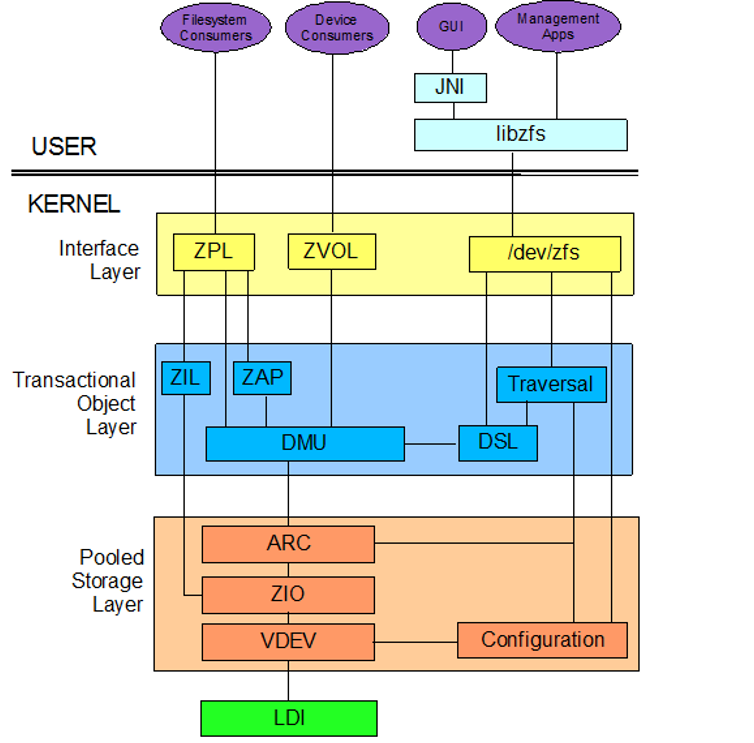
\includegraphics[width=0.47\linewidth]{figs/ZFS-stack.png}
  % \caption{xxxx}
    \end{figure}  
\end{frame}
%----------------------------------------------
% ##### ZFS I/O Stack
% 
% %% figure
% 	\begin{figure}
% 	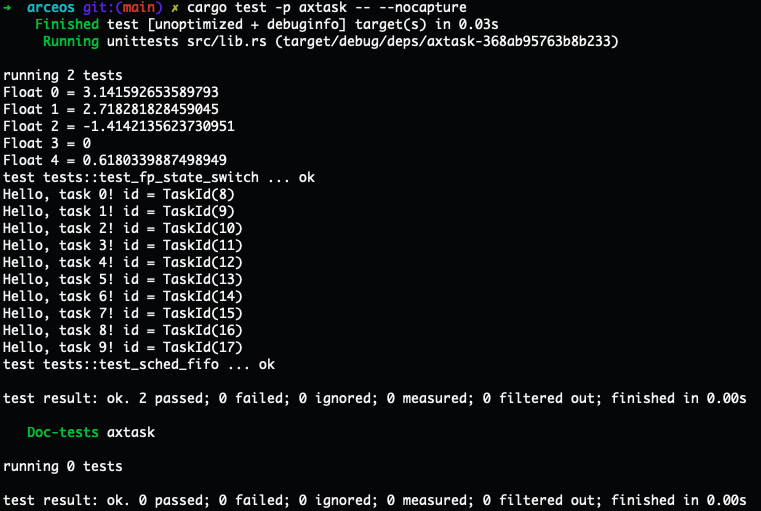
\includegraphics[width=0.8\linewidth]{test}
% %	\caption{xxxx}
% 	\end{figure}
% ![ZFS-stack](figs/ZFS-stack.png)
% 
%----------------------------------------------
\begin{frame}[fragile]
    \frametitle{FS/Volume Model vs. ZFS}
%    \framesubtitle{xxxx}
%% figure
    \begin{figure}
    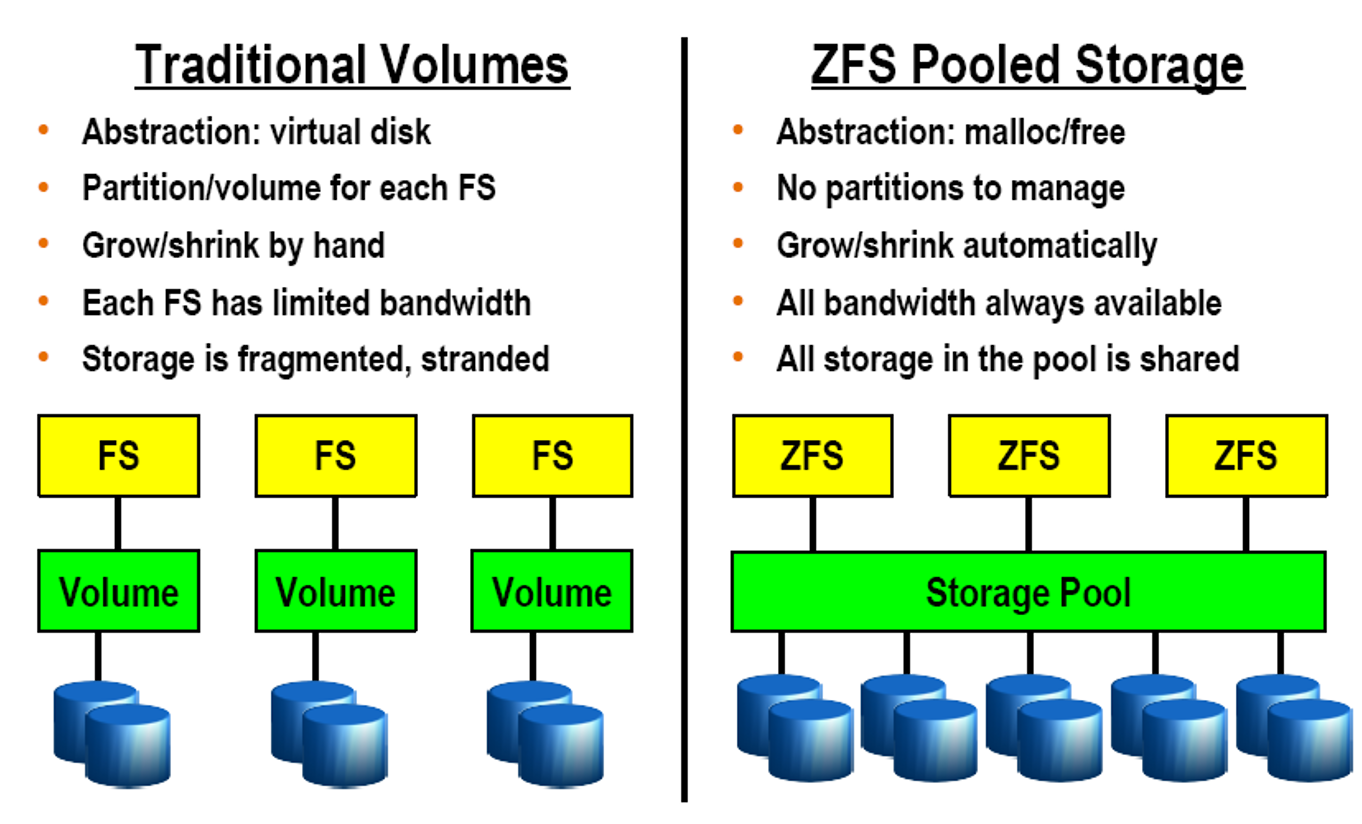
\includegraphics[width=0.8\linewidth]{figs/ZFS-pooled-storage.png}
  % \caption{xxxx}
    \end{figure}
\end{frame}
%----------------------------------------------
% ##### FS/Volume Model vs. ZFS
% 
% %% figure
% 	\begin{figure}
% 	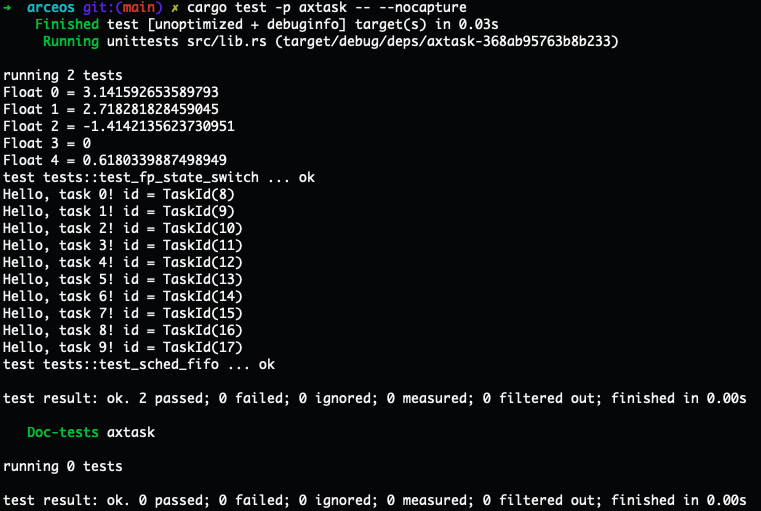
\includegraphics[width=0.8\linewidth]{test}
% %	\caption{xxxx}
% 	\end{figure}
% ![ZFS-pooled-storage](figs/ZFS-pooled-storage.png)
% 
% 
% 
%----------------------------------------------
\begin{frame}[fragile]
    \frametitle{FS/Volume Interfaces vs. ZFS}
%    \framesubtitle{xxxx}
%% figure
    \begin{figure}
    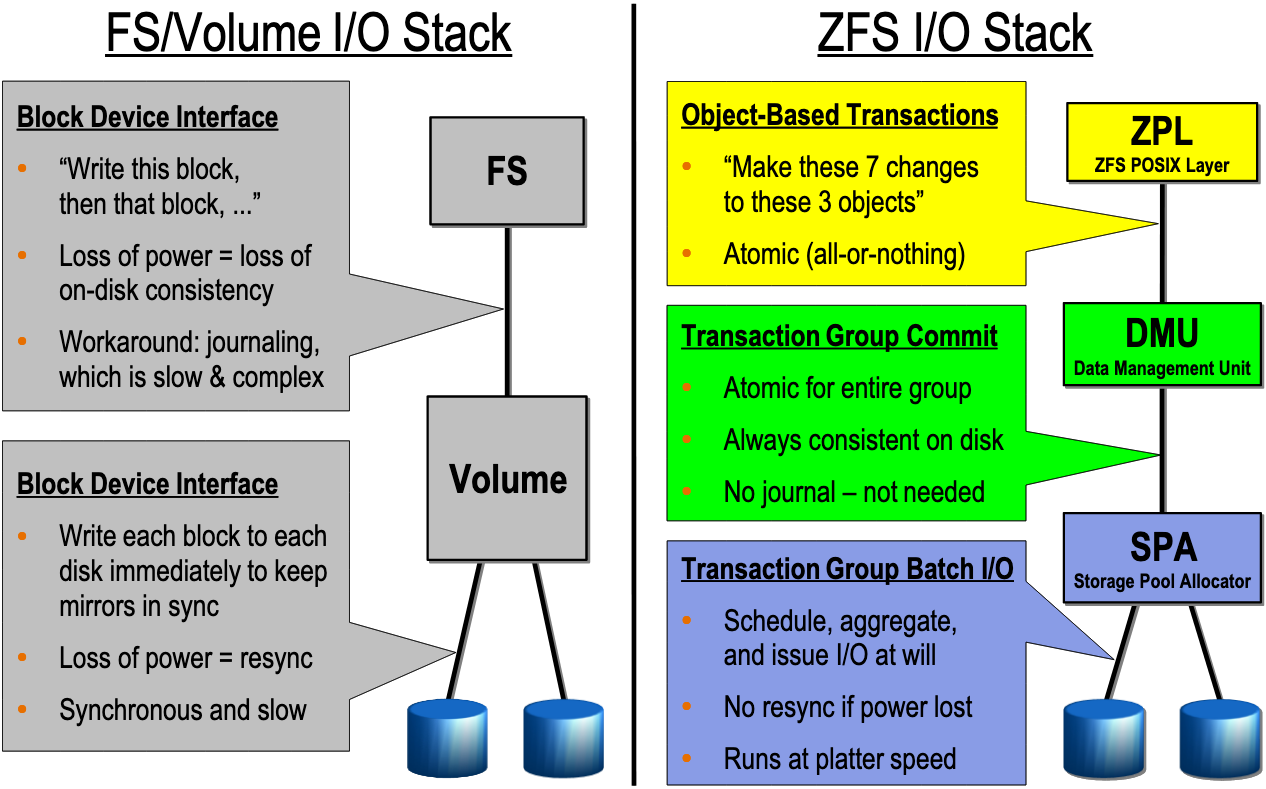
\includegraphics[width=0.7\linewidth]{figs/ZFS-io-stack.png}
  % \caption{xxxx}
    \end{figure}
\end{frame}
%----------------------------------------------
% #### ZFS I/O Stack
% 
% ##### FS/Volume Interfaces vs. ZFS
% 
% %% figure
% 	\begin{figure}
% 	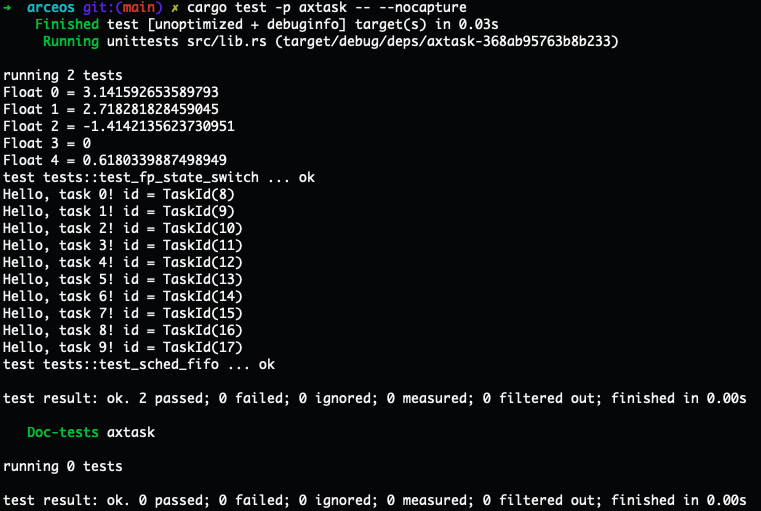
\includegraphics[width=0.8\linewidth]{test}
% %	\caption{xxxx}
% 	\end{figure}
% ![ZFS-io-stack](figs/ZFS-io-stack.png)
% 
%----------------------------------------------
\begin{frame}[fragile]
    \frametitle{ZFL (ZFS POSIX Layer)}
%    \framesubtitle{xxxx}
    \begin{figure}
    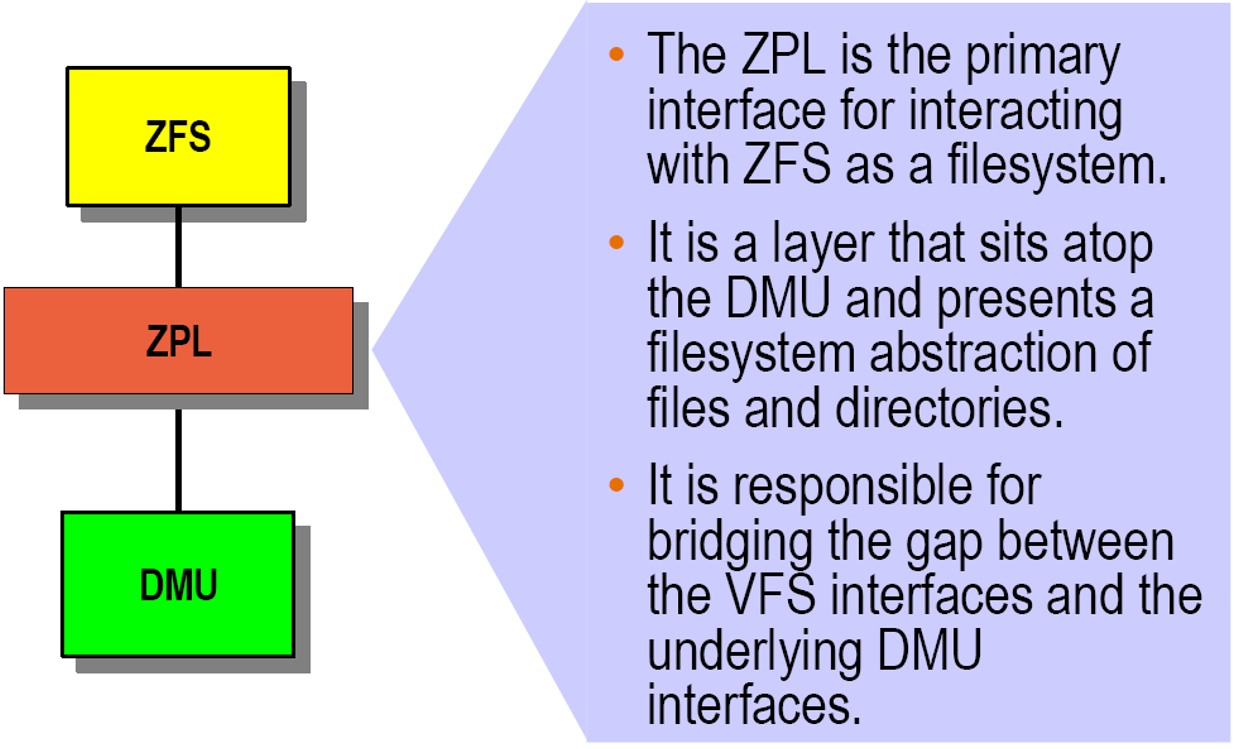
\includegraphics[width=0.75\linewidth]{figs/ZFS-zpl.png}
  % \caption{xxxx}
    \end{figure}  
\end{frame}
%----------------------------------------------
% ##### ZFL (ZFS POSIX Layer)
% 
% %% figure
% 	\begin{figure}
% 	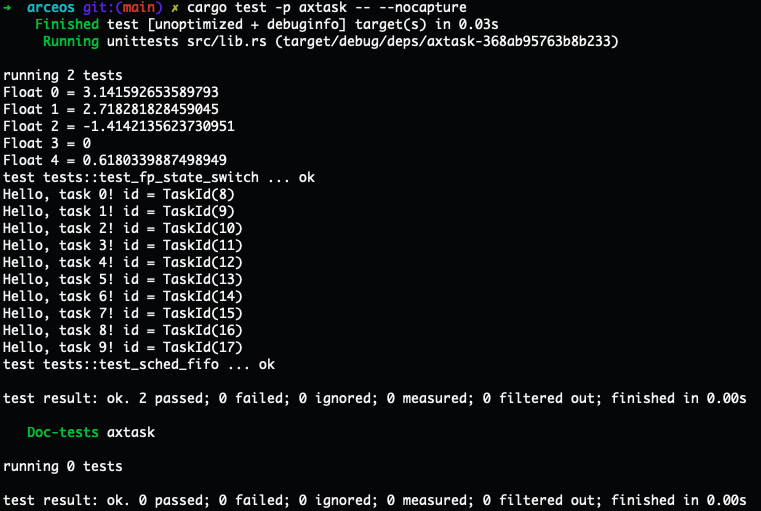
\includegraphics[width=0.8\linewidth]{test}
% %	\caption{xxxx}
% 	\end{figure}
% ![ZFS-zpl](figs/ZFS-zpl.png)
% 
%----------------------------------------------
\begin{frame}[fragile]
    \frametitle{DMU (Data Management Unit)}
%    \framesubtitle{xxxx}
    \begin{figure}
    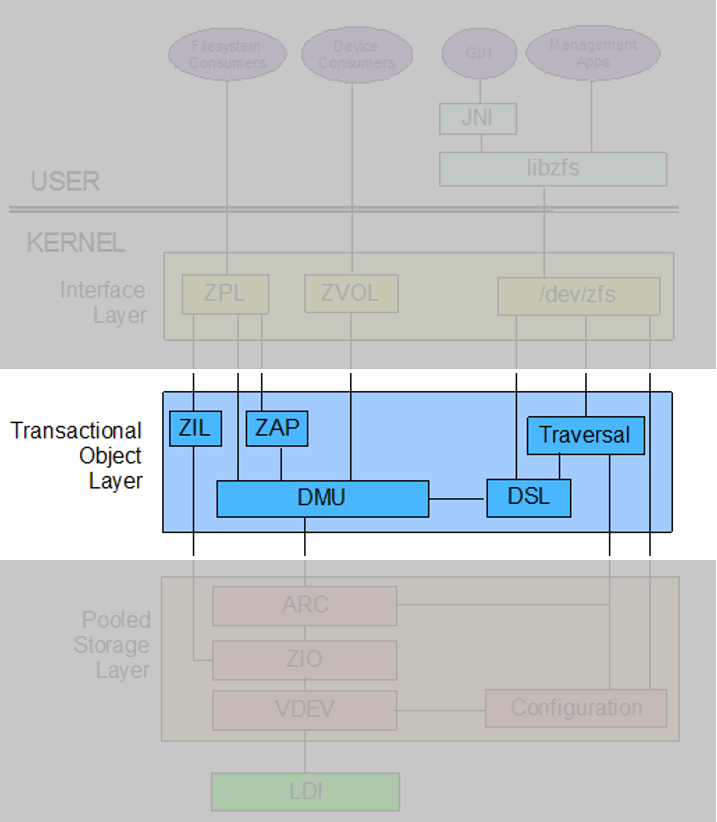
\includegraphics[width=0.75\linewidth]{figs/ZFS-dmu.png}
  % \caption{xxxx}
    \end{figure}
\end{frame}
%----------------------------------------------
% ##### DMU (Data Management Unit)
% 
% %% figure
% 	\begin{figure}
% 	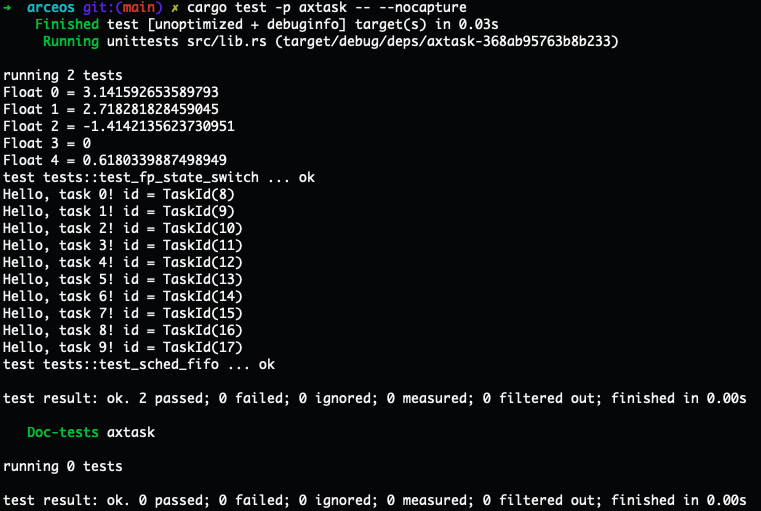
\includegraphics[width=0.8\linewidth]{test}
% %	\caption{xxxx}
% 	\end{figure}
% ![ZFS-dmu](figs/ZFS-dmu.png)
% 
%----------------------------------------------
\begin{frame}[fragile]
    \frametitle{ARC (Adaptive Replacement Cache)}
%    \framesubtitle{xxxx}
    \begin{figure}
    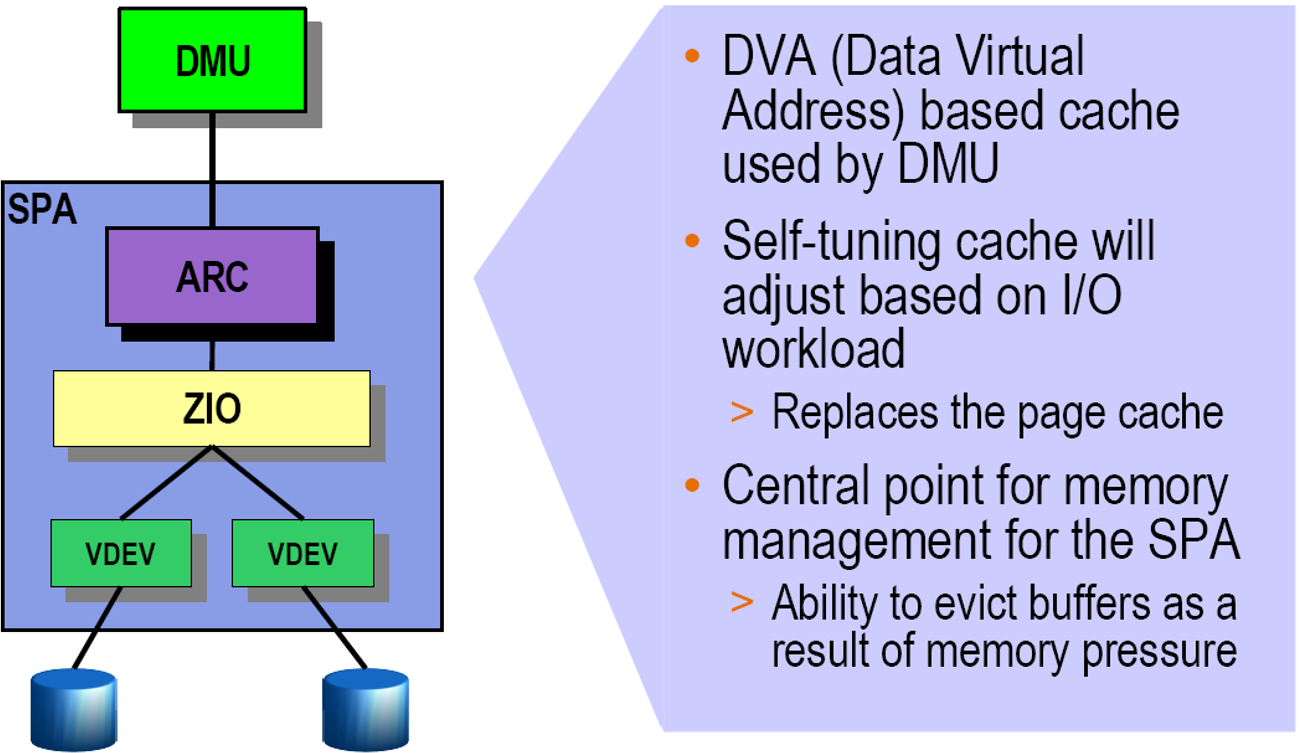
\includegraphics[width=0.8\linewidth]{figs/ZFS-arc.png}
  % \caption{xxxx}
    \end{figure}
\end{frame}
%----------------------------------------------
% ##### ARC (Adaptive Replacement Cache)
% 
% %% figure
% 	\begin{figure}
% 	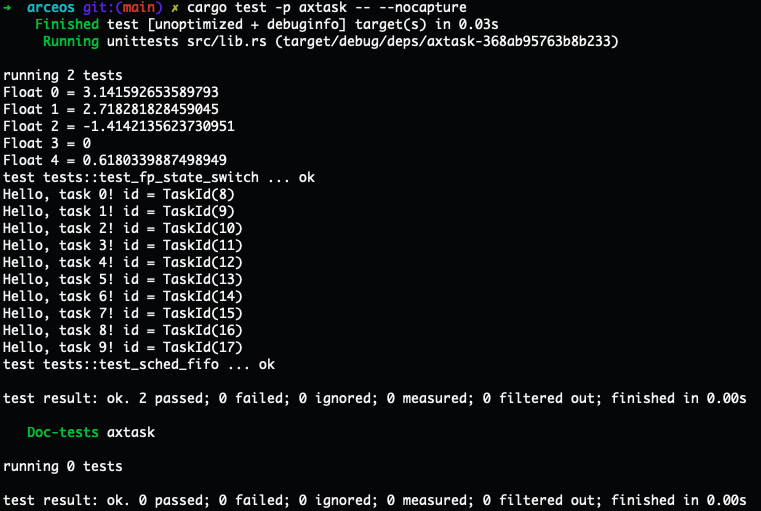
\includegraphics[width=0.8\linewidth]{test}
% %	\caption{xxxx}
% 	\end{figure}
% ![ZFS-arc](figs/ZFS-arc.png)
% 
%----------------------------------------------
\begin{frame}[fragile]
    \frametitle{ZIO (ZFS I/O Pipeline)}
%    \framesubtitle{xxxx}
    \begin{figure}
    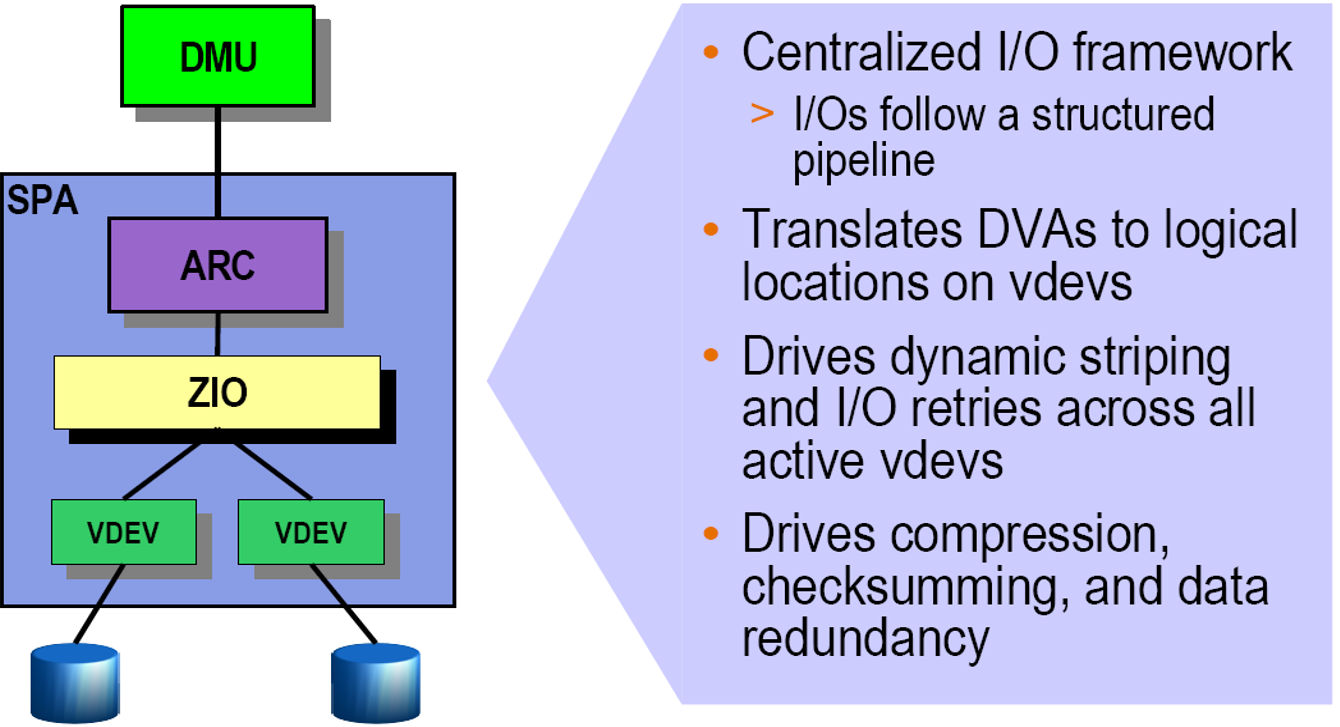
\includegraphics[width=0.85\linewidth]{figs/ZFS-zio.png}
  % \caption{xxxx}
    \end{figure}
\end{frame}
%----------------------------------------------
% ##### ZIO (ZFS I/O Pipeline)
% 
% %% figure
% 	\begin{figure}
% 	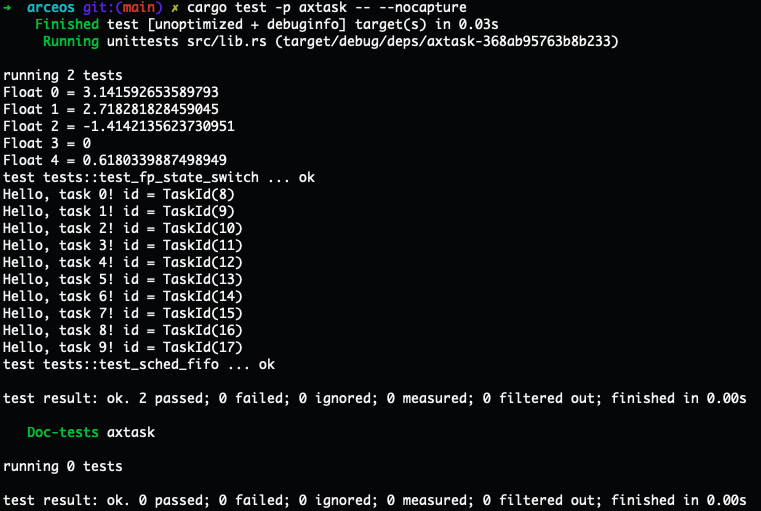
\includegraphics[width=0.8\linewidth]{test}
% %	\caption{xxxx}
% 	\end{figure}
% ![ZFS-zio](figs/ZFS-zio.png)
% 
%----------------------------------------------
\begin{frame}[fragile]
    \frametitle{VDEV (Virtual Devices)}
%    \framesubtitle{xxxx}
    \begin{figure}
    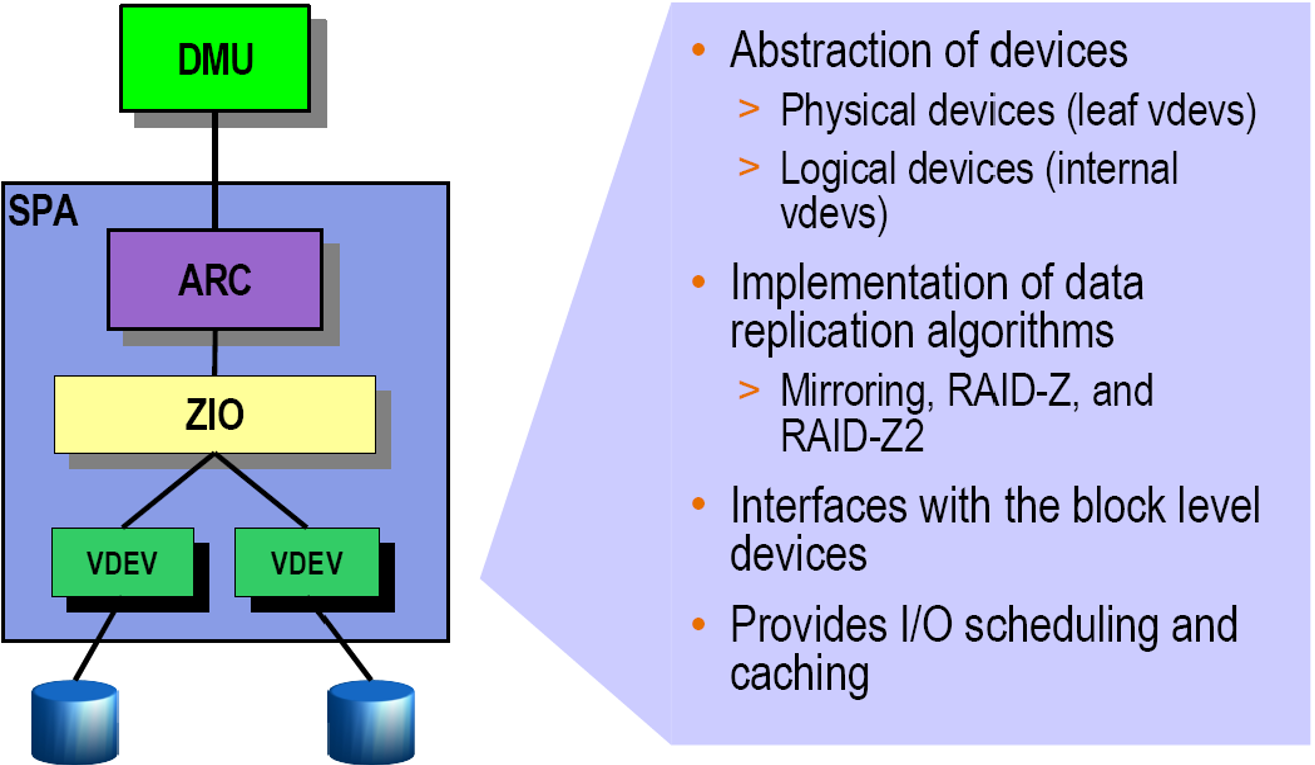
\includegraphics[width=0.8\linewidth]{figs/ZFS-vdev.png}
  % \caption{xxxx}
    \end{figure}
\end{frame}
%----------------------------------------------
% ##### VDEV (Virtual Devices)
% 
% %% figure
% 	\begin{figure}
% 	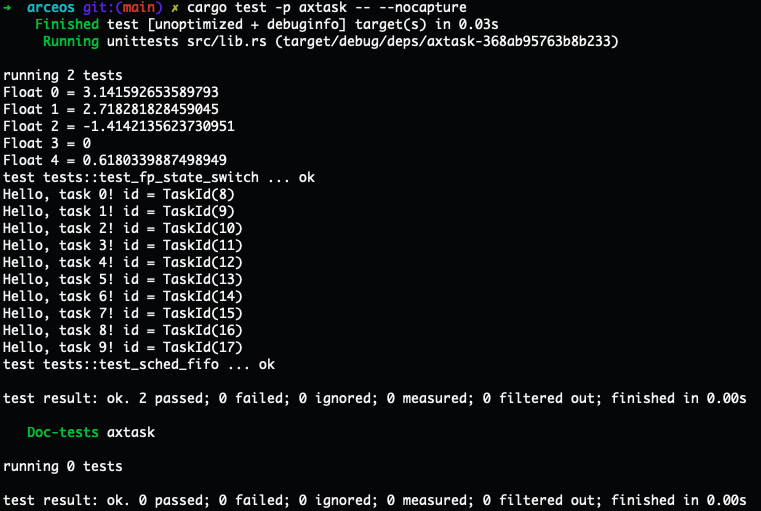
\includegraphics[width=0.8\linewidth]{test}
% %	\caption{xxxx}
% 	\end{figure}
% ![ZFS-vdev](figs/ZFS-vdev.png)
% 
%----------------------------------------------
\begin{frame}
\frametitle{提纲} % Table of contents slide, comment this block out to remove it
\tableofcontents % Throughout your presentation, if you choose to use \section{} and \subsection{} commands, these will automatically be printed on this slide as an overview of your presentation
\end{frame}
%----------------------------------------------
\subsection{ZFS Data Integrity Model} % A subsection can be created just before a set of slides with a common theme to further break down your presentation into chunks
%----------------------------------------------
\begin{frame}[fragile]
    \frametitle{ZFS Data Integrity Model}
%    \framesubtitle{xxxx}
%% itemize
    \begin{itemize}
        \item Everything is copy-on-write
        \begin{itemize}
            \item Never overwrite live data
            \item On-disk state always valid – no “windows of vulnerability”
            \item No need for fsck(1M)
        \end{itemize} \pause
        \item Everything is transactional
        \begin{itemize}
            \item Related changes succeed or fail as a whole
            \item No need for journaling
        \end{itemize} \pause
        \item Everything is checksummed
        \begin{itemize}
            \item No silent data corruption
        \end{itemize}
    \end{itemize}
\end{frame}
%----------------------------------------------
% #### ZFS Data Integrity Model
% 
% 
% 
% ##### ZFS Data Integrity Model
% 
% %% itemize
%     \begin{itemize}
%         \item xx
%     \end{itemize}
%  * Everything is copy-on-write
%     * Never overwrite live data
%     * On-disk state always valid – no “windows of vulnerability”
%     * No need for fsck(1M)
%  * Everything is transactional
%     * Related changes succeed or fail as a whole
%     * No need for journaling
%  * Everything is checksummed
%     * No silent data corruption
% 
%----------------------------------------------
\begin{frame}[fragile]
    \frametitle{Copy-On-Write Transactions}
%    \framesubtitle{xxxx}
    \begin{figure}
    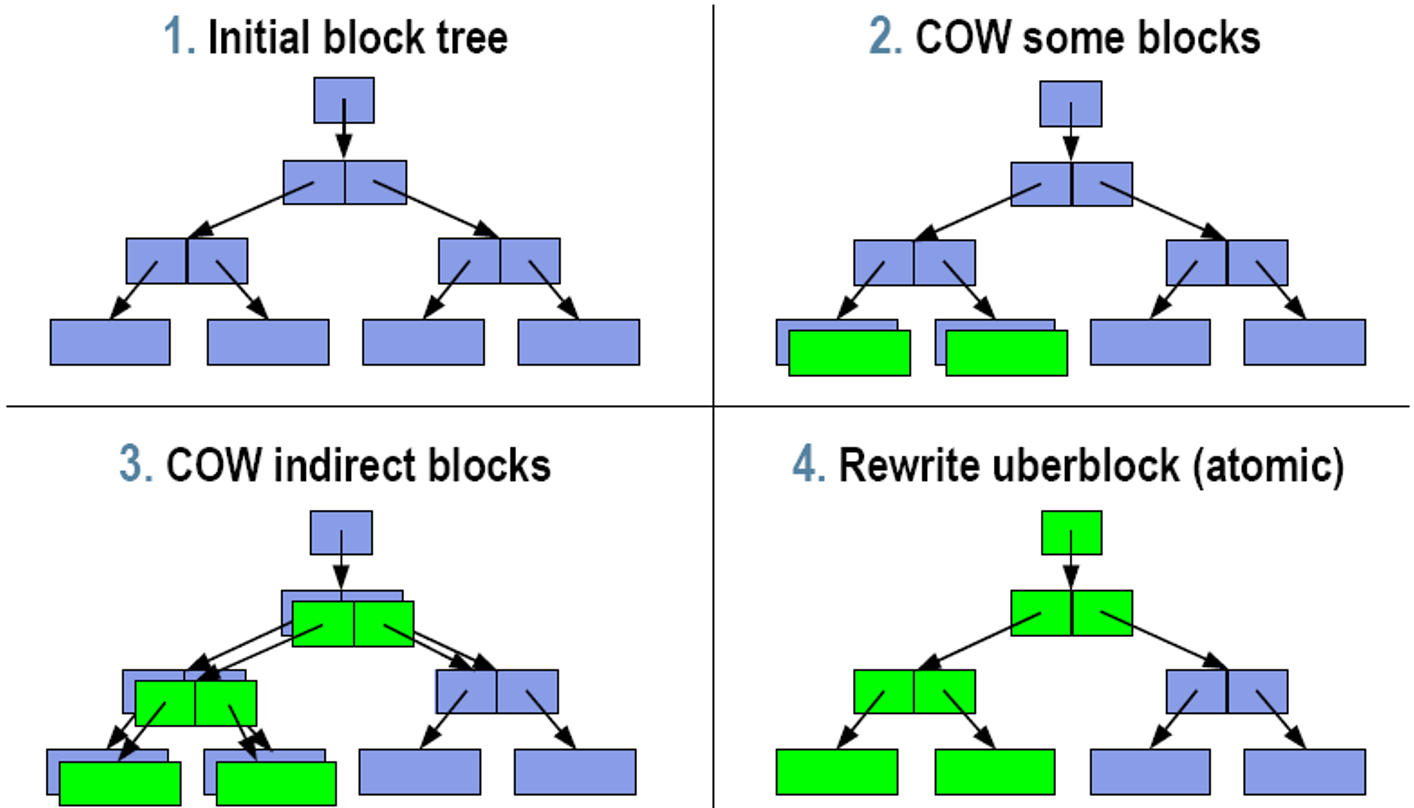
\includegraphics[width=0.8\linewidth]{figs/ZFS-cow.png}
  % \caption{xxxx}
    \end{figure}
\end{frame}
%----------------------------------------------
% ##### Copy-On-Write Transactions
% 
% %% figure
% 	\begin{figure}
% 	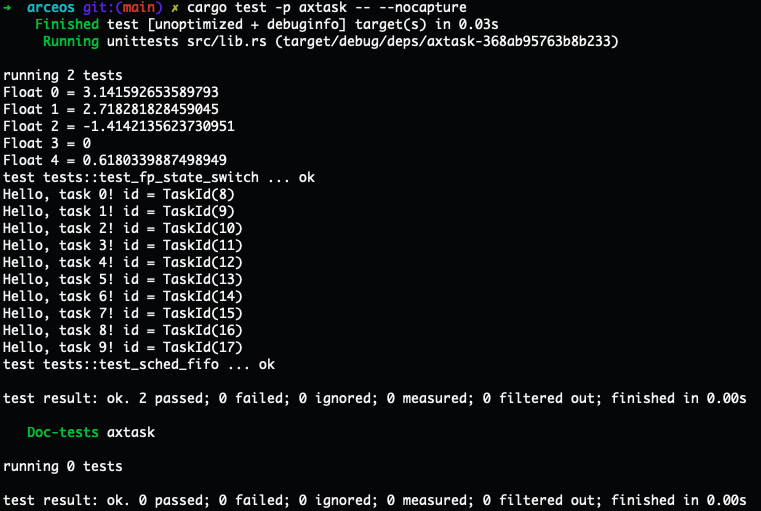
\includegraphics[width=0.8\linewidth]{test}
% %	\caption{xxxx}
% 	\end{figure}
% ![ZFS-cow](figs/ZFS-cow.png)
% 
%----------------------------------------------
\begin{frame}[fragile]
    \frametitle{Constant-Time Snapshots}
%    \framesubtitle{xxxx}
    \begin{figure}
    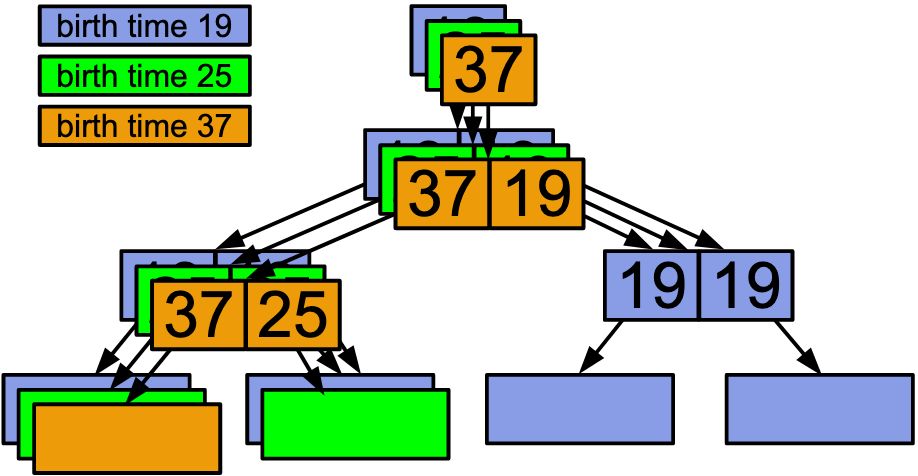
\includegraphics[width=0.6\linewidth]{figs/ZFS-snapshot2.png}
  % \caption{xxxx}
    \end{figure}
%% itemize
    \begin{itemize}
        \item At end of TX group, don't free COWed blocks
        \begin{itemize}
            \item Actually cheaper to take a snapshot than not!
        \end{itemize}
        \item The tricky part:  how do you know when a block is free?
    \end{itemize}
\end{frame}
%----------------------------------------------
% ##### Constant-Time Snapshots
% Ref: http://pages.cs.wisc.edu/~remzi/OSTEP/Citations/zfs_last.pdf - Page 11
% http://pages.cs.wisc.edu/~remzi/OSTEP/Citations/zfs_last.pdf P10
% 
% %% figure
% 	\begin{figure}
% 	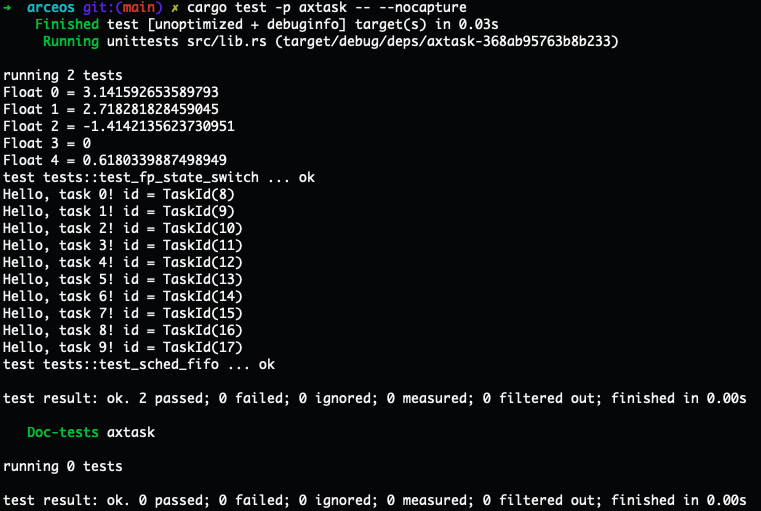
\includegraphics[width=0.8\linewidth]{test}
% %	\caption{xxxx}
% 	\end{figure}
% ![ZFS-snapshot](figs/ZFS-snapshot2.png)
% 
% At end of TX group, don't free COWed blocks
% 
% Actually cheaper to take a snapshot than not!
% 
% The tricky part:  how do you know when a block is free?
% 
% 
% 
%----------------------------------------------
\begin{frame}[fragile]
    \frametitle{End-to-End Checksums}
%    \framesubtitle{xxxx}
    \begin{figure}
    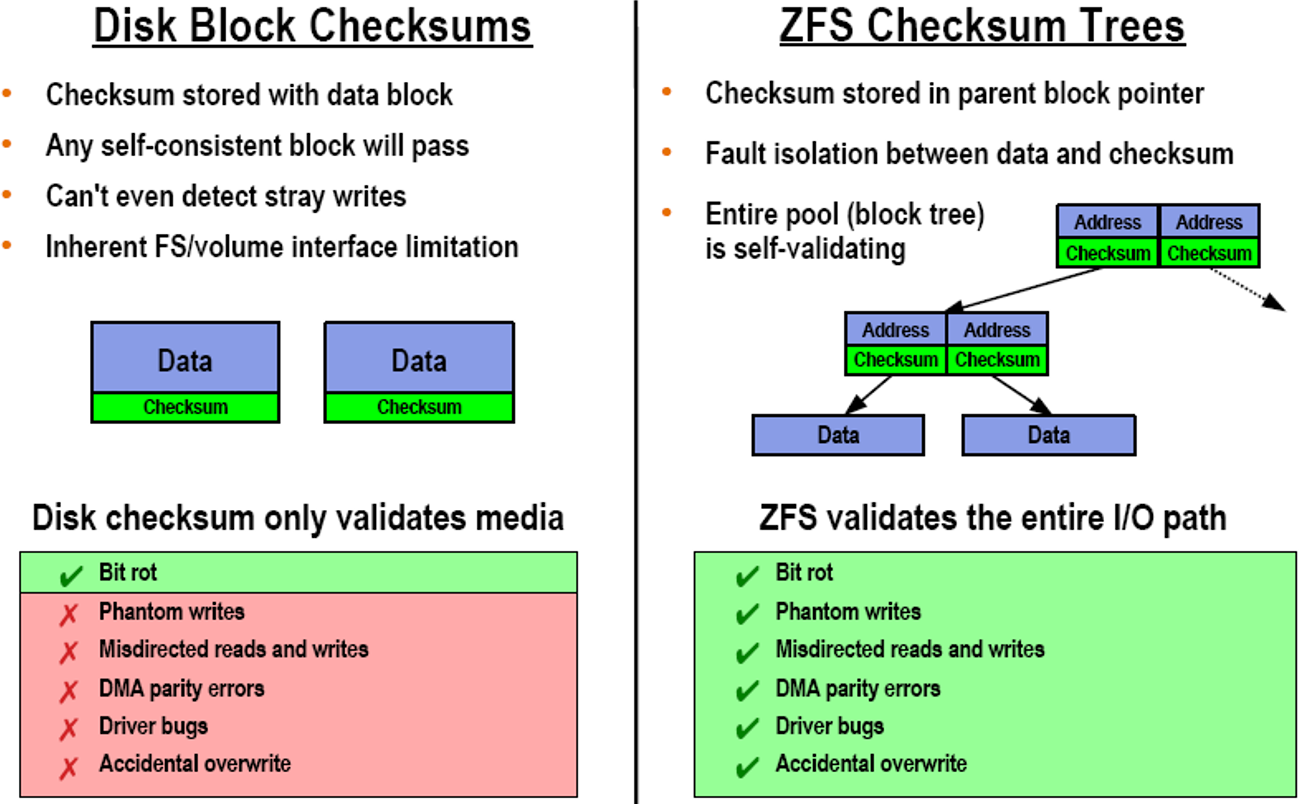
\includegraphics[width=0.7\linewidth]{figs/ZFS-checksum.png}
  % \caption{xxxx}
    \end{figure}
\end{frame}
%----------------------------------------------
% ##### End-to-End Checksums
% 
% %% figure
% 	\begin{figure}
% 	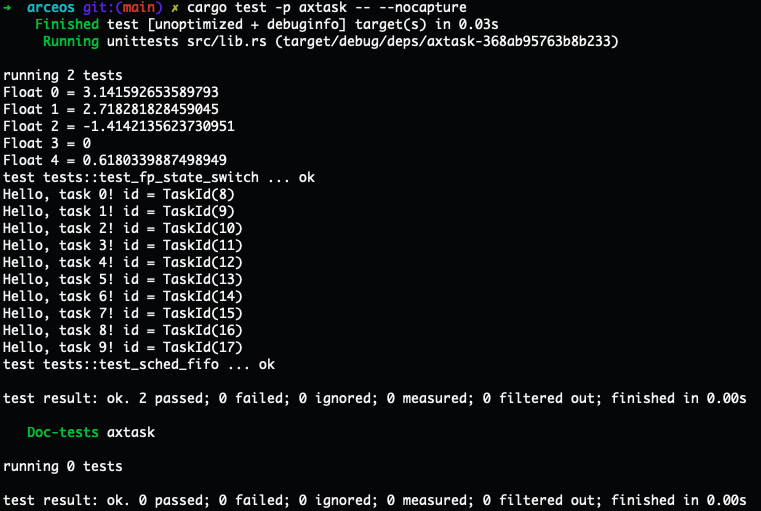
\includegraphics[width=0.8\linewidth]{test}
% %	\caption{xxxx}
% 	\end{figure}
% ![ZFS-checksum](figs/ZFS-checksum.png)
% 
%----------------------------------------------
\begin{frame}[fragile]
    \frametitle{Self-Healing Data in ZFS}
%    \framesubtitle{xxxx}
    \begin{figure}
    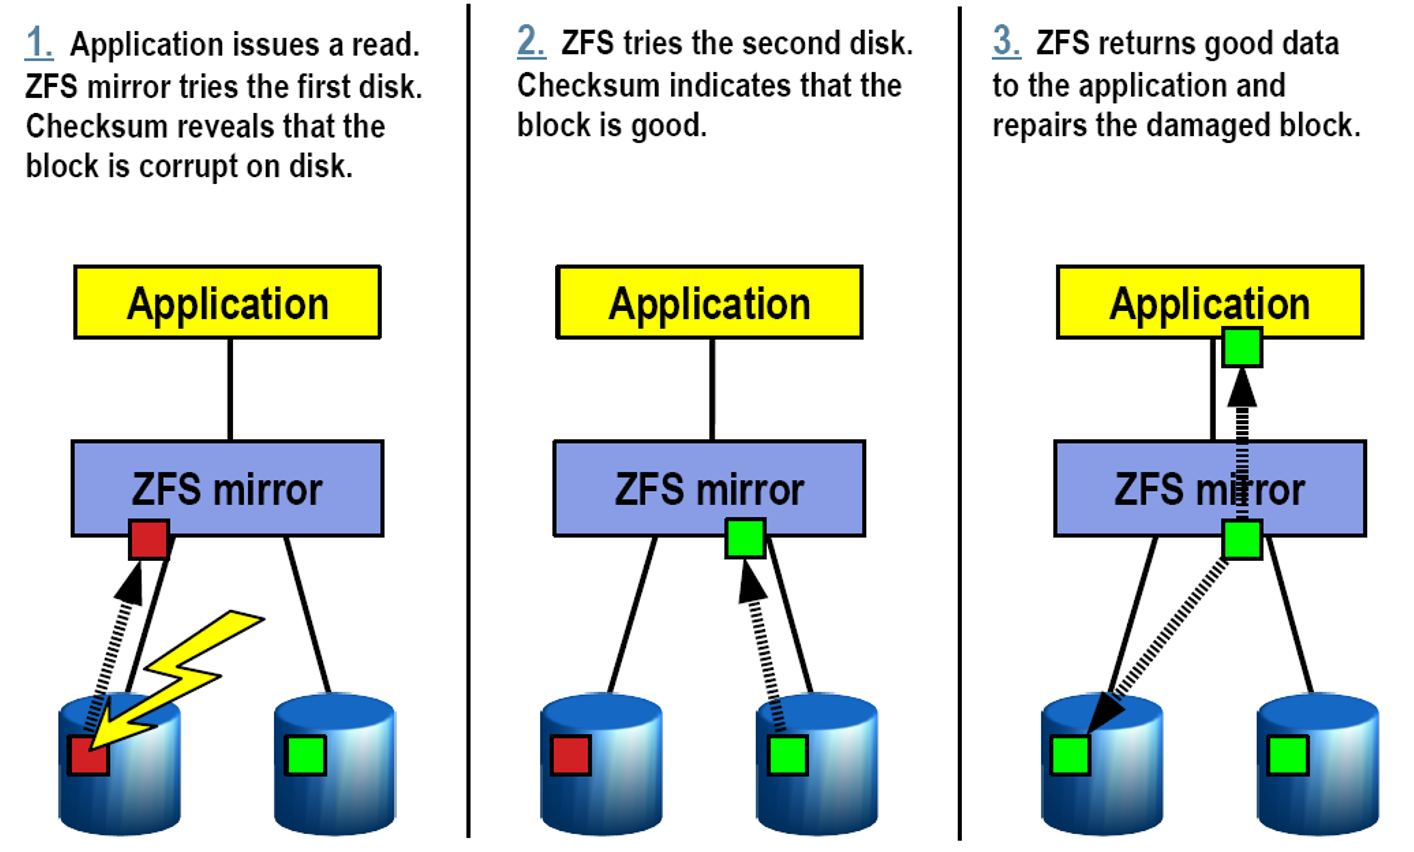
\includegraphics[width=0.8\linewidth]{figs/ZFS-self-healing.png}
  % \caption{xxxx}
    \end{figure}
\end{frame}
%----------------------------------------------
% ##### Self-Healing Data in ZFS
% 
% %% figure
% 	\begin{figure}
% 	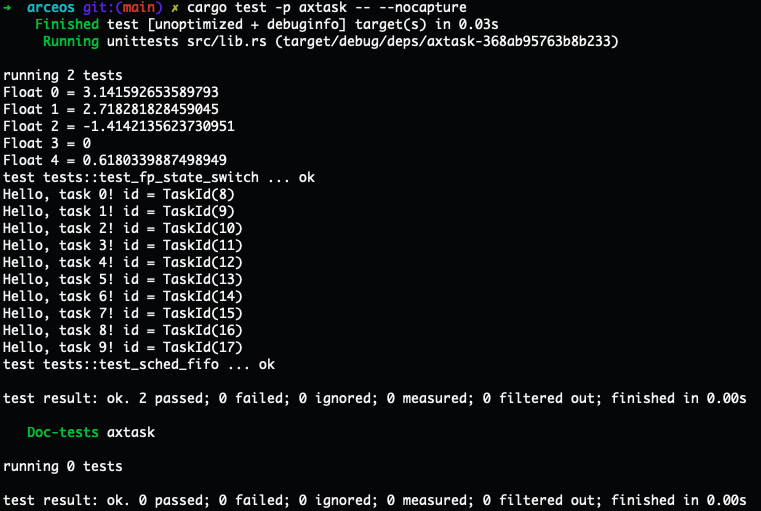
\includegraphics[width=0.8\linewidth]{test}
% %	\caption{xxxx}
% 	\end{figure}
% ![ZFS-self-healing](figs/ZFS-self-healing.png)
% 
%----------------------------------------------
\begin{frame}[fragile]
    \frametitle{RAID-Z}
%% columns
      \begin{columns}
      \begin{column}{0.4\textwidth}
%       \framesubtitle{xxxx}
        \begin{figure}
        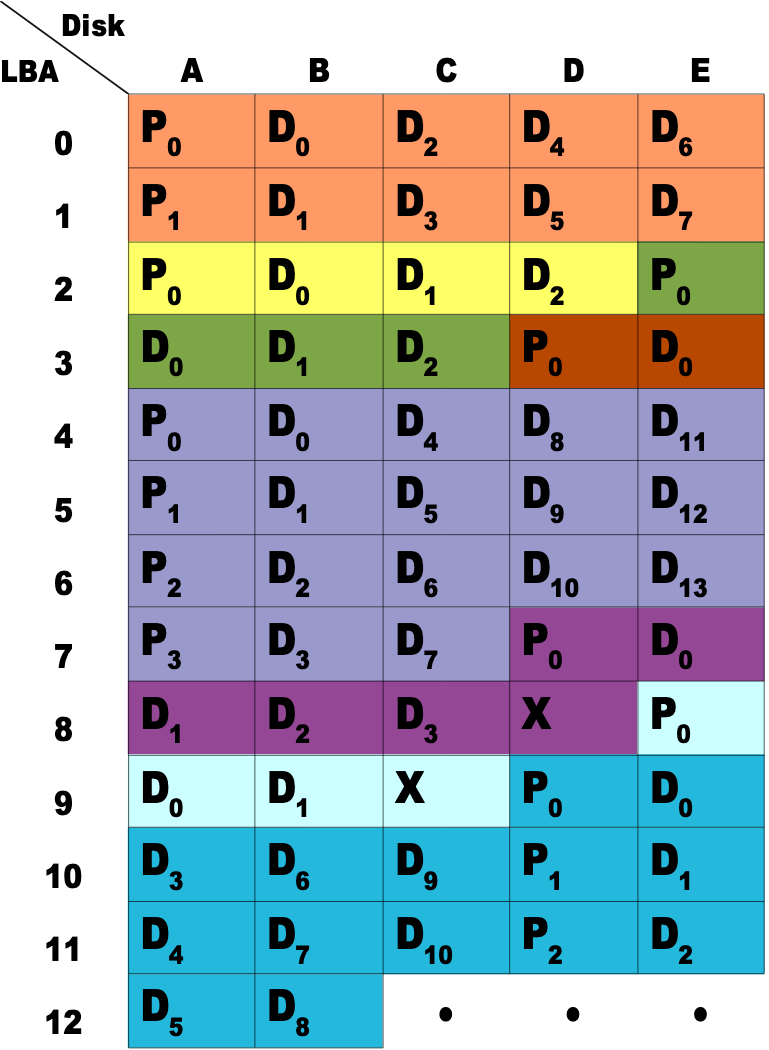
\includegraphics[width=0.8\linewidth]{figs/ZFS-raidz.png}
      % \caption{xxxx}
        \end{figure}
      \end{column}
      \begin{column}{0.6\textwidth}
    %% itemize
        \begin{itemize}
            \item Dynamic stripe width
            \begin{itemize}
                \item Variable block size: 512–128K
                \item Each logical block is its own stripe
            \end{itemize} \pause
            \item All writes are full-stripe writes
            \begin{itemize}
                \item Eliminates read-modify-write (it's fast)
                \item Eliminates the RAID-5 write hole(no need for NVRAM)
            \end{itemize} \pause
            \item Both single and double parity
            \item Detects and corrects silent data corruption
            \begin{itemize}
                \item Checksum-driven combinatorial reconstruction
            \end{itemize} \pause
            \item {\color{red}No special hardware}–ZFS loves cheap disks
        \end{itemize}
      \end{column}
      \end{columns}
\end{frame}
%----------------------------------------------
% ##### RAID-Z
% 
% Ref: http://pages.cs.wisc.edu/~remzi/OSTEP/Citations/zfs_last.pdf Page 18
% 
% %% figure
% 	\begin{figure}
% 	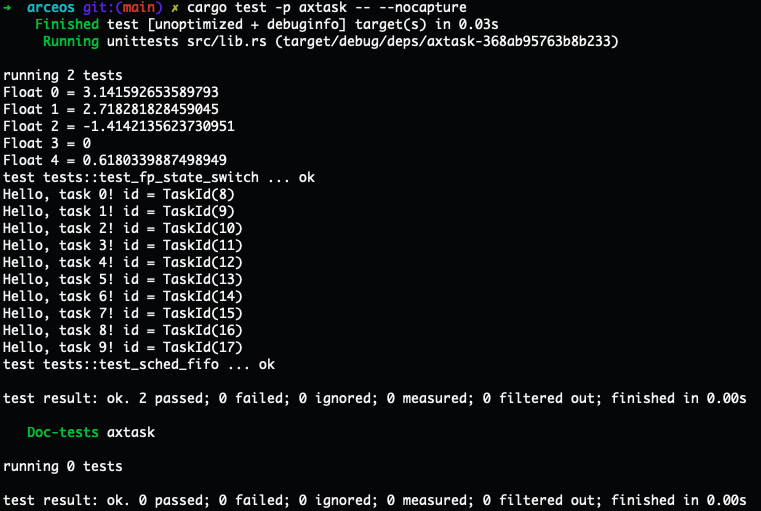
\includegraphics[width=0.8\linewidth]{test}
% %	\caption{xxxx}
% 	\end{figure}
% ![ZFS-raidz](figs/ZFS-raidz.png)
% 
% %% itemize
%     \begin{itemize}
%         \item xx
%     \end{itemize}
%  * Dynamic stripe width
%     * Variable block size: 512 – 128K
%     * Each logical block is its own stripe
%  * All writes are full-stripe writes
%     * Eliminates read-modify-write (it's fast)
%     * Eliminates the RAID-5 write hole(no need for NVRAM)
%  * Both single- and double-parity
%  * Detects and corrects silent data corruption
%     * Checksum-driven combinatorial reconstruction
%  * **No special hardware** – ZFS loves cheap disks
% 
%----------------------------------------------
\begin{frame}[fragile]
    \frametitle{Dynamic Striping}
%    \framesubtitle{xxxx}
    \begin{figure}
    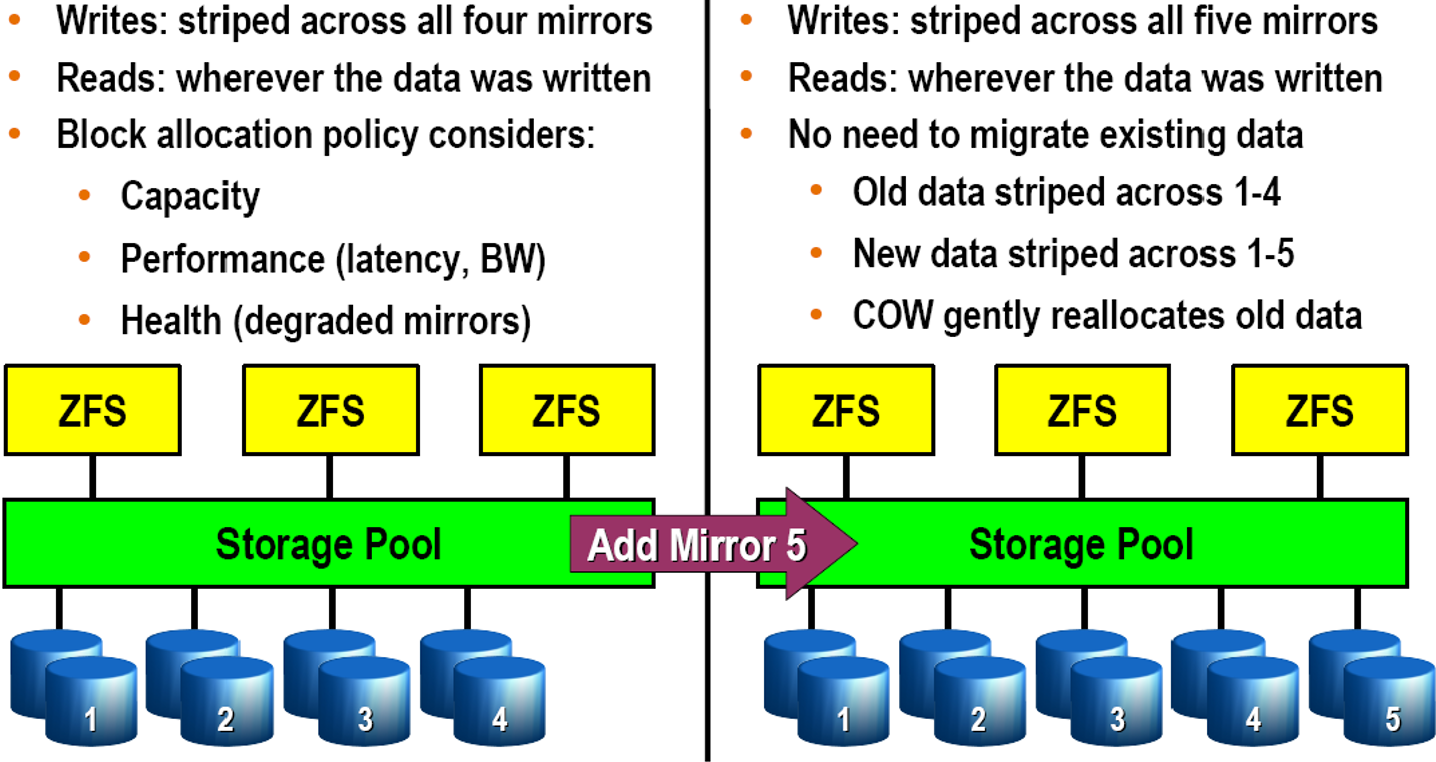
\includegraphics[width=0.8\linewidth]{figs/ZFS-striping.png}
  % \caption{xxxx}
    \end{figure}
\end{frame}
%----------------------------------------------
% ##### Dynamic Striping
% 
% Automatically distributes load across all devices
% 
% %% figure
% 	\begin{figure}
% 	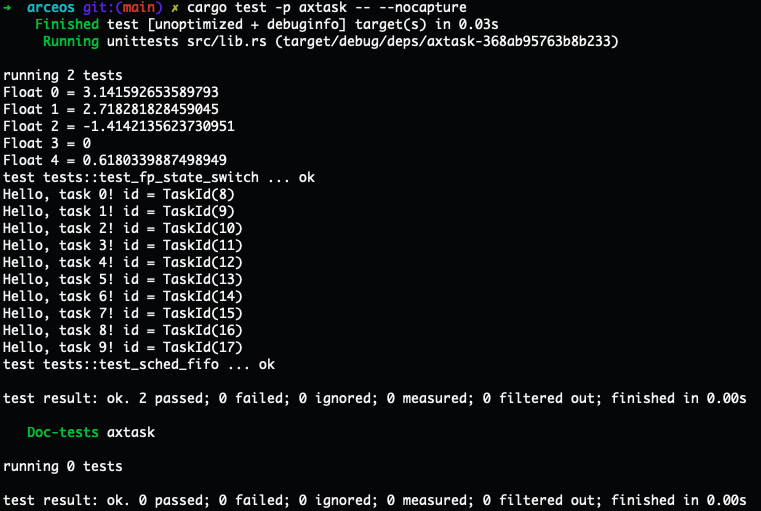
\includegraphics[width=0.8\linewidth]{test}
% %	\caption{xxxx}
% 	\end{figure}
% ![ZFS-striping](figs/ZFS-striping.png)
% 
%----------------------------------------------
\begin{frame}[fragile]
    \frametitle{Object-Based Storage}
%    \framesubtitle{xxxx}
    \begin{figure}
    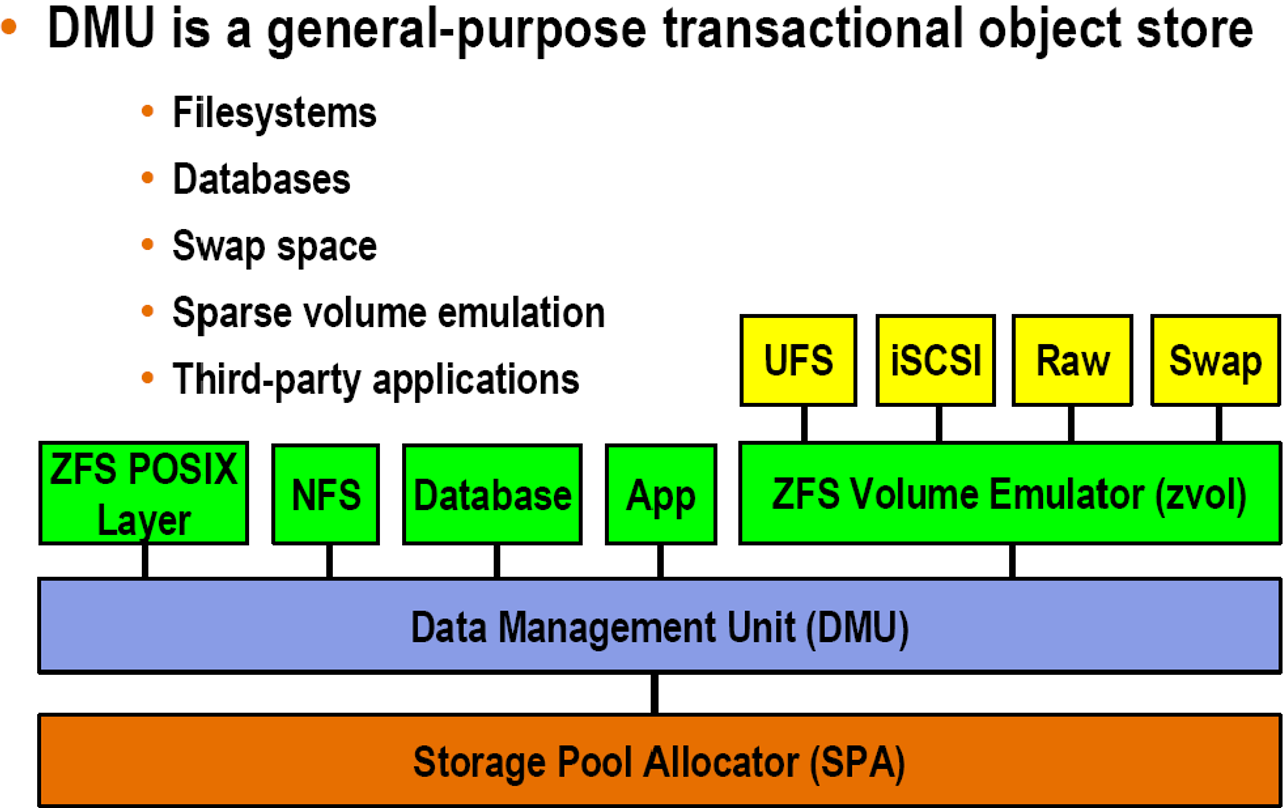
\includegraphics[width=0.7\linewidth]{figs/ZFS-storage.png}
  % \caption{xxxx}
    \end{figure}

\end{frame}
%----------------------------------------------
% ##### Object-Based Storage
% 
% %% figure
% 	\begin{figure}
% 	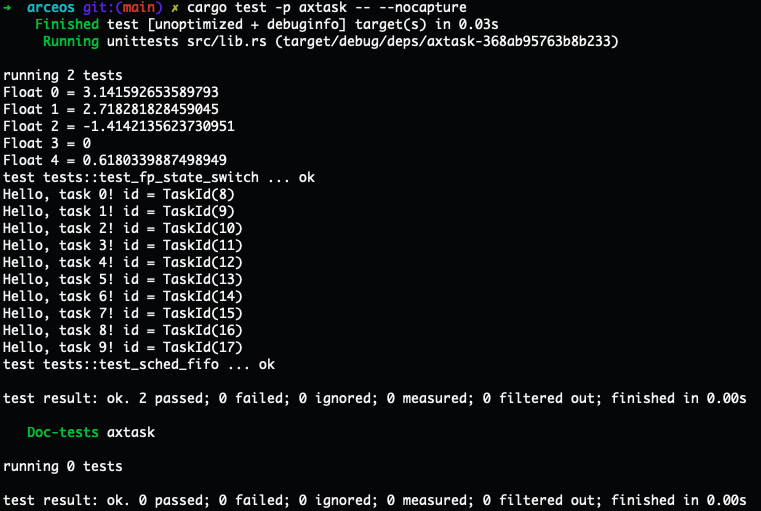
\includegraphics[width=0.8\linewidth]{test}
% %	\caption{xxxx}
% 	\end{figure}
% ![ZFS-storage](figs/ZFS-storage.png)
% 
% 
% 
%----------------------------------------------
\begin{frame}[fragile]
    \frametitle{Variable Block Size}
%    \framesubtitle{xxxx}
%% itemize
    \begin{itemize}
        \item No single block size is optimal for everything
        \begin{itemize}
            \item Large blocks: less metadata, higher bandwidth
            \item Small blocks: more space-efficient for small objects
            \item Record-structured files (e.g. databases) have natural granularity; filesystem must match it to avoid read/modify/write
        \end{itemize} \pause
        \item Per-object granularity
        \begin{itemize}
            \item A 37k file consumes 37k – no wasted space
        \end{itemize}
        \item Enables transparent block-based compression
    \end{itemize}
\end{frame}
%----------------------------------------------
% ##### Variable Block Size
% 
% Ref: http://pages.cs.wisc.edu/~remzi/OSTEP/Citations/zfs_last.pdf Page 28
% 
% %% itemize
%     \begin{itemize}
%         \item xx
%     \end{itemize}
%  * No single block size is optimal for everything
%     * Large blocks: less metadata, higher bandwidth
%     * Small blocks: more space-efficient for small objects
%     * Record-structured files (e.g. databases) have natural granularity; filesystem must match it to avoid read/modify/write
%  * Per-object granularity
%     * A 37k file consumes 37k – no wasted space
%  * Enables transparent block-based compression
% 
%----------------------------------------------
\begin{frame}[fragile]
    \frametitle{Built-in Compression}
%    \framesubtitle{xxxx}
    \begin{figure}
    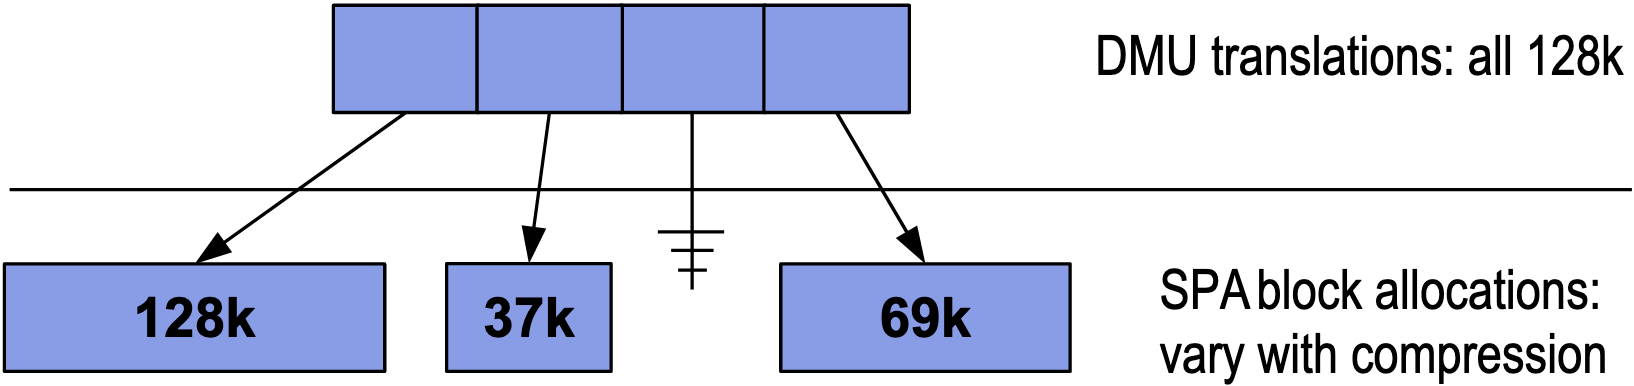
\includegraphics[width=0.8\linewidth]{figs/ZFS-compression.png}
  % \caption{xxxx}
    \end{figure}
%% itemize
    \begin{itemize}
        \item Block-level compression in SPA
        \item Transparent to all other layers \pause
        \item Each block compressed independently
        \item All-zero blocks converted into file holes
        \item LZJB and GZIP available today; more on the way
    \end{itemize}
\end{frame}
%----------------------------------------------
% ##### Built-in Compression
% 
% Ref: http://pages.cs.wisc.edu/~remzi/OSTEP/Citations/zfs_last.pdf Page 29
% 
% %% figure
% 	\begin{figure}
% 	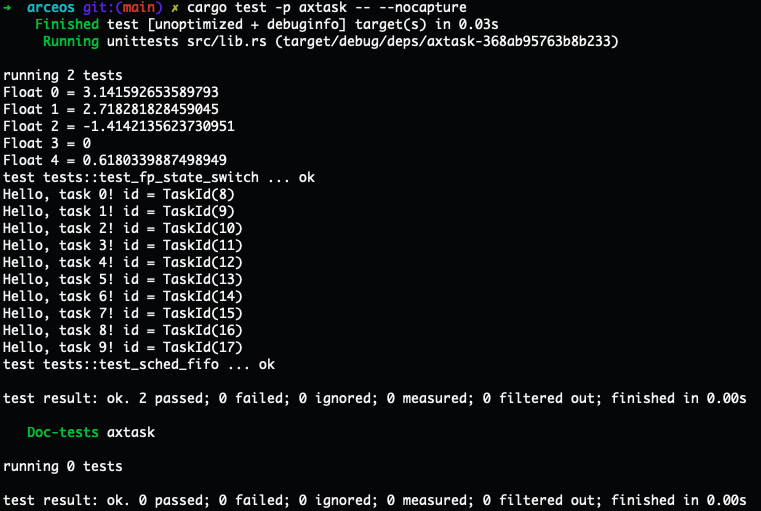
\includegraphics[width=0.8\linewidth]{test}
% %	\caption{xxxx}
% 	\end{figure}
% ![ZFS-compression](figs/ZFS-compression.png)
% 
% %% itemize
%     \begin{itemize}
%         \item xx
%     \end{itemize}
%  * Block-level compression in SPA
%  * Transparent to all other layers
%  * Each block compressed independently
%  * All-zero blocks converted into file holes
%  * LZJB and GZIP available today; more on the way
%----------------------------------------------
\end{document}
